\documentclass[12pt, a4paper]{article}
\usepackage[T2A]{fontenc}
\usepackage[utf8x]{inputenc}
\usepackage[english, russian]{babel}
\usepackage{mathtools}
\DeclareMathOperator{\arcsinh}{arcsinh}
\DeclareMathOperator{\arccosh}{arccosh}
\DeclareMathOperator{\arctanh}{arctanh}
\DeclareMathOperator{\arccoth}{arccoth}
\begin{document}
\title{Производная туда сюда
}\author{Севсоль, 1 курс ЭРТЭ}
\date{\today}
\maketitle 
\centerline{Разложим в окрестности 0 по формуле тейлора до $\tilde{o}(x^9)$ вот такую функцию} 
\begin{equation}
f(x) = \sin(x)
\end{equation}
\begin{equation}
{f}^{(1)}(x) = \cos(x)\end{equation}\begin{equation}
{f}^{(2)}(x) = -1 \cdot \sin(x)\end{equation}\begin{equation}
{f}^{(3)}(x) = \cos(x) \cdot -1\end{equation}\begin{equation}
{f}^{(4)}(x) = -1 \cdot \sin(x) \cdot -1\end{equation}\begin{equation}
{f}^{(5)}(x) = \cos(x) \cdot -1 \cdot -1\end{equation}\begin{equation}
{f}^{(6)}(x) = -1 \cdot \sin(x) \cdot -1 \cdot -1\end{equation}\begin{equation}
{f}^{(7)}(x) = \cos(x) \cdot -1 \cdot -1 \cdot -1\end{equation}\begin{equation}
{f}^{(8)}(x) = -1 \cdot \sin(x) \cdot -1 \cdot -1 \cdot -1\end{equation}\begin{equation}
{f}^{(9)}(x) = \cos(x) \cdot -1 \cdot -1 \cdot -1 \cdot -1\end{equation}\center{Итоговая формула разложения по Тейлору}
\begin{equation}f(x) = x+\frac{-1 \cdot {x}^{3}}{6}+\frac{{x}^{5}}{120}+\frac{-1 \cdot {x}^{7}}{5040}+\frac{{x}^{9}}{362880} + \tilde{o}(x^9)
\end{equation}\center{График исходной функции}
\begin{center}
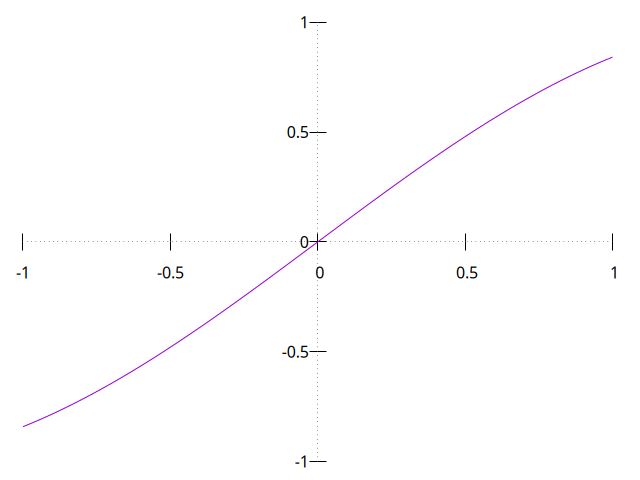
\includegraphics[scale=0.5]{start_func.png}
\end{center}
\center{График разложения по тейлору функции}
\begin{center}
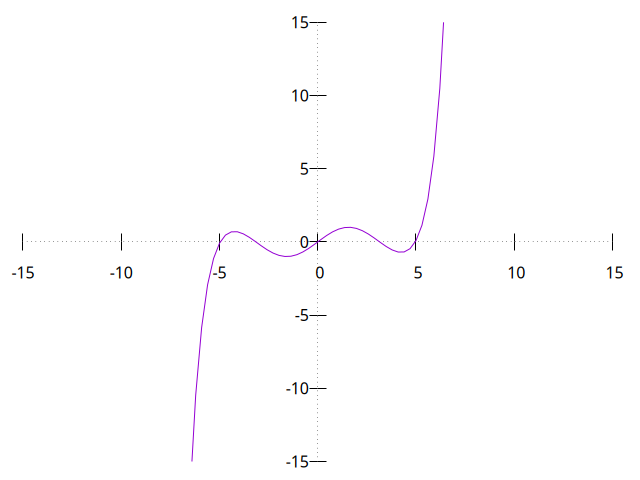
\includegraphics[scale=0.5]{taylor_formula.png}
\end{center}
\center{График разницы между исходной функцией и разложением по Тейлору}
\begin{center}
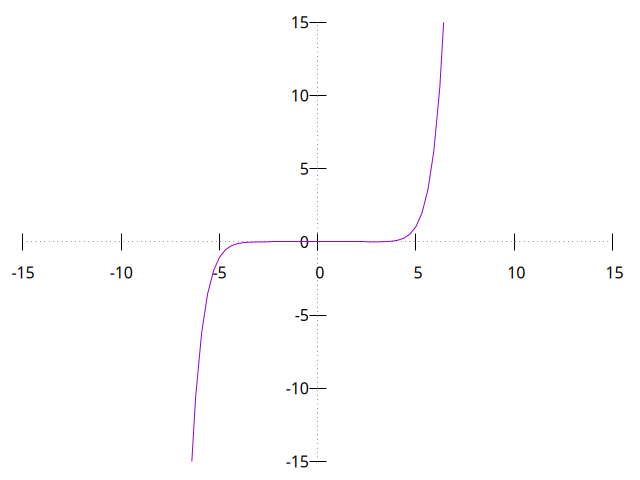
\includegraphics[scale=0.5]{delta.png}
\end{center}

\end{document}
